\documentclass{beamer}
\usetheme[pageofpages=of,% String used between the current page and the
                         % total page count.
          bullet=circle,% Use circles instead of squares for bullets.
          titleline=true,% Show a line below the frame title.
          alternativetitlepage=true,% Use the fancy title page.
       %   titlepagelogo=logo-polito,% Logo for the first page.
       %   watermark=watermark-polito,% Watermark used in every page.
       %   watermarkheight=100px,% Height of the watermark.
       %   watermarkheightmult=4,% The watermark image is 4 times bigger
                                % than watermarkheight.
          ]{Torino}

\setbeamertemplate{footline}{
  \begin{beamercolorbox}[wd=\paperwidth,ht=1ex,dp=1ex]{footline}
    \vspace{5pt} \hspace{1em} \insertframenumber/\inserttotalframenumber
  \end{beamercolorbox}
}

\author{Brendon J. Brewer}
\title{STATS 331 -- Introduction to Bayesian Statistics}
\institute{The University of Auckland}
\date{}


\linespread{1.3}
\usepackage{minted}
\usepackage[utf8]{inputenc}
\usepackage{dsfont}
\newcommand{\given}{\,|\,}

\begin{document}

\frame{\titlepage}

\begin{frame}
\begin{center}
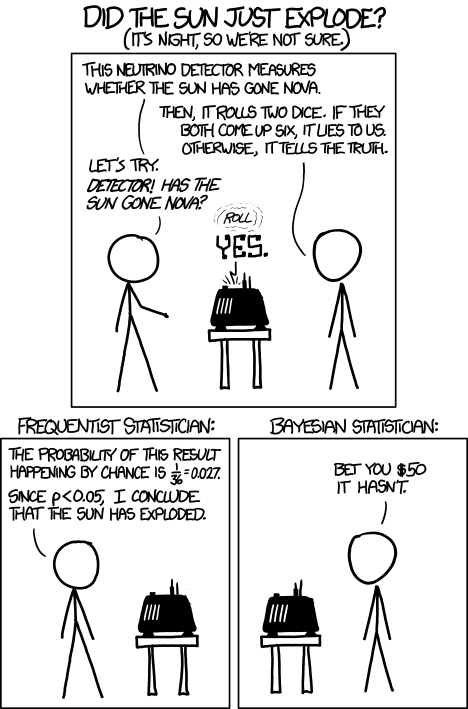
\includegraphics[width=0.4\textwidth]{images/xkcd.png} \\
Credit: Randall Monroe, xkcd
\end{center}

\end{frame}

\begin{frame}
\begin{center}
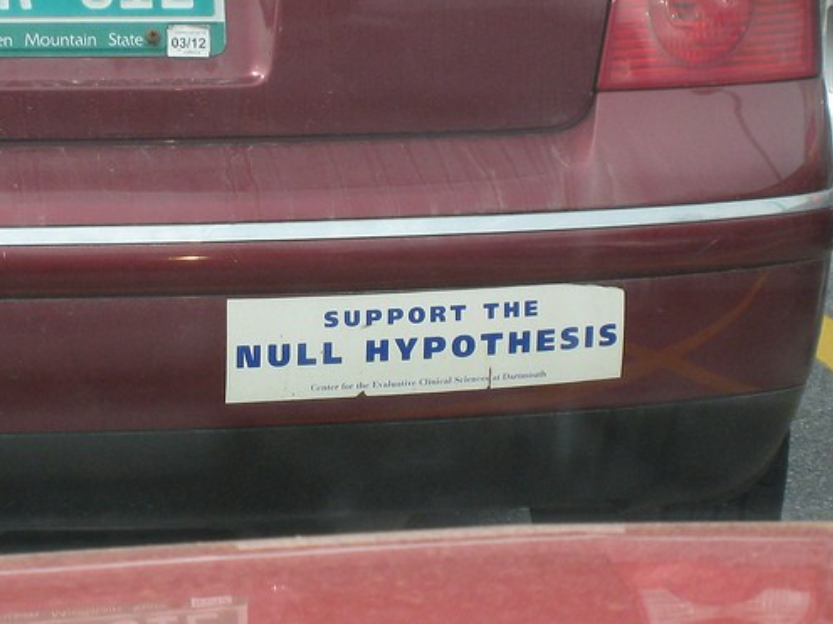
\includegraphics[width=0.6\textwidth]{images/support_null.png} \\
Credit: Unknown
\end{center}

\end{frame}

\begin{frame}
\begin{center}
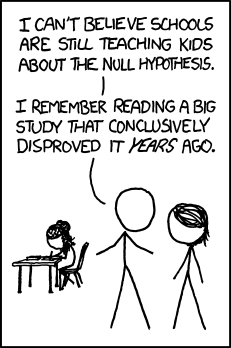
\includegraphics[width=0.4\textwidth]{images/null_hypothesis.png} \\
Credit: Randall Monroe, xkcd
\end{center}

\end{frame}


\begin{frame}
\frametitle{A Hypothesis Testing Scenario}
What if we considered these two hypotheses, as statisticians often do:
\begin{align}
H_0: \theta = 0.5 \\
H_1: \theta \neq 0.5
\end{align}
\pause

There might be a good reason to suspect the `null hypothesis' is true ---
e.g. if the effect being studied is absent.\pause

Classical/frequentist statistics would use {\bf p-values} for this, but we
will not.
\end{frame}


\begin{frame}
\frametitle{Hypothesis Testing vs. Parameter Estimation}
When we write down a list of hypotheses and get their
posterior probabilities (e.g., in a Bayes' Box), we have tested all of the
hypotheses using the data. So there is not much else to do.
\pause
\begin{itemize}
\item In classical statistics, estimation and hypothesis testing
are quite distinct and are approached using different techniques.\pause
\item For us, they're basically the same thing --- except sometimes we will use a
different prior.
\end{itemize}

\end{frame}


\begin{frame}
\frametitle{Ed Jaynes Quote}

    \begin{columns} % Create two columns
        \column{0.5\textwidth} % Left column (50% width)
        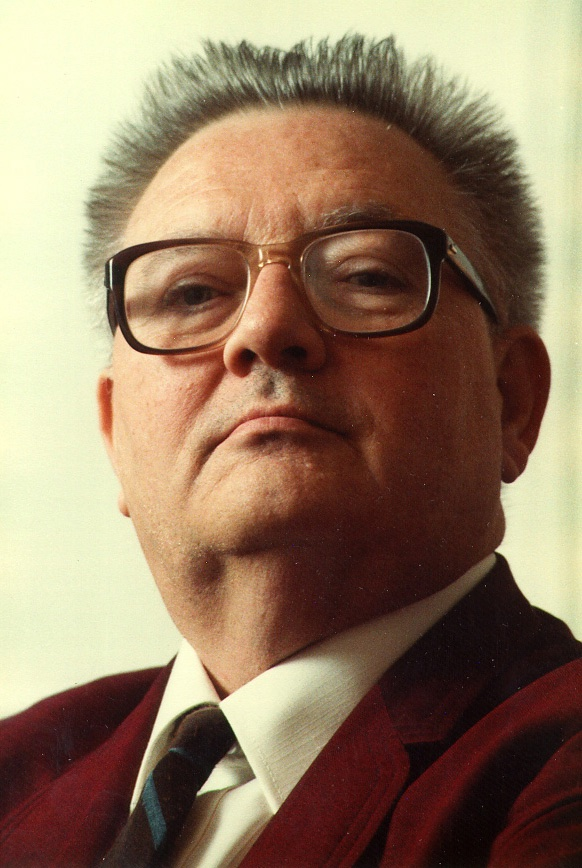
\includegraphics[width=0.7\linewidth]{images/jaynes.jpg}

        \column{0.5\textwidth} % Right column (50% width)
        {\em ``Any hypothesis testing
procedure can be
replaced by a parameter
estimation procedure that
is simpler and more
informative.''}
     \end{columns}

\end{frame}


\begin{frame}
\frametitle{Bus Problem from Lecture Notes}
When I first moved to Auckland, I caught buses arbitrarily, hoping I would
get to the right place. I achieved $x=2$ successes out of $N=5$ trials.
The binomial sampling distribution applies to $x$ here.\pause

Suppose we wanted to test $H_0: \theta = 0.5$. The p-value would be
\begin{align}
\textnormal{p-value} &= P(x \leq 2 \vee x \geq 3 \given H_0) = 1.
\end{align}
\pause
Traditionally, a statistician would say there is no evidence against the null
hypothesis. But is there evidence {\em for} it? In the Bayesian version of
hypothesis testing, we will be able to say that sometimes.

\end{frame}

\begin{frame}
\frametitle{Criticisms of P-Values}
Many people have criticised p-values. Some of the arguments include, but are not
limited to:
\begin{itemize}
\item P-values are not the probability of the null hypothesis, but are sometimes
interpreted as if they were.\pause
\item Frequentist statisticians know they are not. However, they are obviously
an attempt to quantify the plausibility of $H_0$.\pause
\item They do not take into account what you would have expected to observe if
$H_0$ were false.\pause
\item They are based on the probability of data that did not occur
(hypotheses in the tails).
\end{itemize}

\end{frame}

\begin{frame}
\frametitle{Harold Jeffreys Quote}

    \begin{columns} % Create two columns
        \column{0.5\textwidth} % Left column (50% width)
        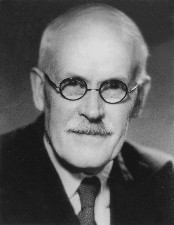
\includegraphics[width=0.7\linewidth]{images/jeffreys.jpg}

        \column{0.5\textwidth} % Right column (50% width)
        {\em ``A hypothesis may be rejected because it has not predicted
               observable results that did not occur!''}
     \end{columns}

\end{frame}

\begin{frame}
\frametitle{Spike and Slab Prior}
For us, the only distinction between a hypothesis testing situation and a
parameter estimation one is that a particular value of the parameter has
been singled out for special attention --- usually because it's plausible.\pause

To take this into account, all we have to do is give the special value of
$\theta$ more prior probability than it would have otherwise. This leads
to a `spike' in the prior. The rest of the $\theta$ values form a `slab'.
\end{frame}


\begin{frame}
\frametitle{Bayes' Box: Uniform Prior}

\centering
{\footnotesize
\begin{tabular}{|c|c|c|c|c|}
\hline
Parameter & Prior & Likelihood & Prior $\times$ Likelihood & Posterior \\
$\theta$  & $p(\theta)$ & $p(x \given \theta)$ & $p(\theta)p(x\given \theta)$ & $p(\theta\given x)$ \\
\hline
0 & 0.0909 &  & & \\
0.1 & 0.0909  &   & & \\
0.2 & 0.0909 &  &  &  \\
0.3 & 0.0909 &  &  &  \\
0.4 & 0.0909 &  &  &  \\
0.5 & 0.0909 &  &  &  \\
0.6 & 0.0909 &  &  &  \\
0.7 & 0.0909 &  &  &  \\
0.8 & 0.0909 &  &  &  \\
0.9 & 0.0909 &  &  &  \\
1 & 0.0909 &  &  &  \\
\hline
Total & 1 & & & 1 \\
\hline
\end{tabular}
}

\end{frame}

\begin{frame}
\frametitle{Bayes' Box: Spike and Slab Prior}

\centering
{\footnotesize
\begin{tabular}{|c|c|c|c|c|}
\hline
Parameter & Prior & Likelihood & Prior $\times$ Likelihood & Posterior \\
$\theta$  & $p(\theta)$ & $p(x \given \theta)$ & $p(\theta)p(x\given \theta)$ & $p(\theta\given x)$ \\
\hline
0 & 0.05 & 0 & 0 & 0\\
0.1 & 0.05 & 0.0729  & 0.003645 & 0.0163\\
0.2 & 0.05 & 0.2048 & 0.01024  & 0.0457 \\
0.3 & 0.05 & 0.3087 & 0.01544 & 0.0689 \\
0.4 & 0.05 & 0.3456 & 0.01728 & 0.0772 \\
{\bf 0.5} & {\bf 0.5} & {\bf 0.3125} & {\bf 0.1563} & {\bf 0.6977} \\
0.6 & 0.05 & 0.2304 & 0.0115 & 0.0514 \\
0.7 & 0.05 & 0.1323 & 0.0662 & 0.0295 \\
0.8 & 0.05 & 0.0512 & 0.00256 & 0.0114 \\
0.9 & 0.05 & 0.0081 & 0.000405 & 0.0018 \\
1 & 0.05 & 0 & 0 & 0 \\
\hline
Total & 1 & & 0.224 & 1 \\
\hline
\end{tabular}
}

\end{frame}

\begin{frame}[fragile]
\frametitle{Constructing the Spike and Slab Prior in R}
You first create the slab, then manually put in the spike.

\begin{minted}{r}
theta = seq(0, 1, by=0.1)
prior = rep(0.5/(length(theta)-1), length(theta))
prior[abs(theta - 0.5) < 1E-7] = 0.5
\end{minted}
\pause

{\bf Note}: Instead of testing for exact equality of the
\mintinline{r}{theta} values to 0.5, I just found the
value close to 0.5. This is more robust due to computer weirdness.
\end{frame}

\begin{frame}[fragile]
\frametitle{Bus Problem Likelihood}
For completeness, here is the likelihood for the bus problem.

\begin{minted}{r}
lik = dbinom(2, size=5, prob=theta)
\end{minted}
\end{frame}


\begin{frame}[fragile]
\frametitle{Key Differences from Frequentist Hypothesis Testing}

\begin{itemize}
\item No p-value. Instead, calculate the posterior probability of the null
hypothesis.\pause
\item This has a clearer interpretation, and is what we really want to know.\pause
\item You can get evidence {\bf for} the null hypothesis, if the data
suggests this. This happened in the bus example we just saw, as the
probability went up from 0.5 to 0.6977.
\end{itemize}

\end{frame}


\begin{frame}[fragile]
\frametitle{Terminology}
In Bayesian hypothesis testing (closely related to `Bayesian model selection'),
there is some additional terminology, and additional quantities that people
like to talk about.\\[0.5em]

Some of these are the {\bf evidence (marginal likelihood)},
the {\bf Bayes factor}, and the {\bf odds ratio}.\\[0.5em]

These re-express the same conclusions that we already have with posterior
probabilities, but in a different form.

\end{frame}


\begin{frame}
\frametitle{Bayes' Rule Twice}
Here is Bayes' rule twice, expressing the posterior probabilities of two
hypotheses $H_0$ and $H_1$:
\begin{align}
P(H_0 \given x) &= \frac{P(H_0)p(x \given H_0)}{p(x)} \\
P(H_1 \given x) &= \frac{P(H_1)p(x \given H_1)}{p(x)}
\end{align}
\pause

{\bf Note}: I have written upper case $P$ for the terms that are
definitely probabilities, and lower case for the ones that might
be probabilities or probability densities.


\end{frame}


\begin{frame}
\frametitle{Division}
If we divide the two equations by each other, the denominators cancel out,
leaving us with ``Bayes' rule in odds form'':
\begin{align}
\frac{P(H_0 \given x)}{P(H_1 \given x)}
    &= \frac{P(H_0)}{P(H_1)} \times \frac{p(x \given H_0)}{p(x \given H_1)}.
\end{align}
\pause
or
\begin{align}
\textnormal{posterior odds} &=
    \textnormal{prior odds} \times \textnormal{Bayes factor}.
\end{align}


\end{frame}


\begin{frame}
\frametitle{Bus Result Expressed Differently}
\begin{itemize}
\item In the bus problem, the prior probability of $H_0$ was 0.5, so the prior
odds ratio was $0.5/(1 - 0.5) = 1$. The posterior probability was
0.6977 so the posterior odds ratio was $0.6977/(1 - 0.6977)=2.308$.\pause
\item That is, the data makes $H_0$ 2.308 times more probable than $H_1$.\pause
\item We can also solve for the Bayes' factor, which must equal the posterior
odds ratio because the prior odds ratio was 1. Therefore the Bayes' factor
is also 2.308 --- the data was 2.308 times more probable under $H_0$ than
under $H_1$.
\end{itemize}


\end{frame}


\begin{frame}
\frametitle{MacKay Biased Coin Example}

\begin{center}
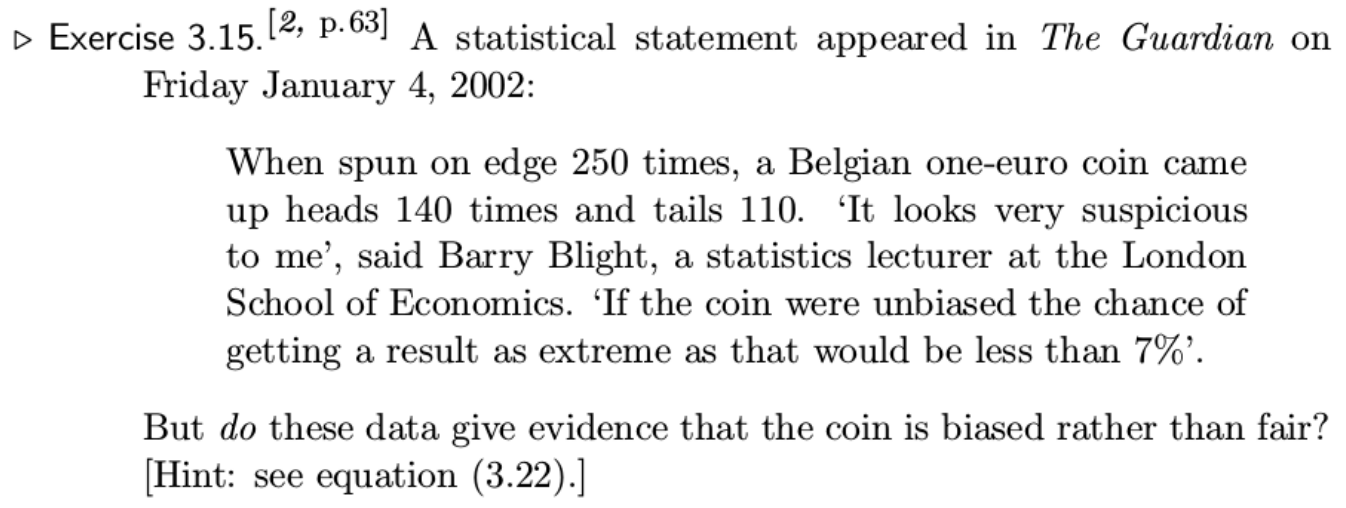
\includegraphics[width=0.9\textwidth]{images/mackay_coin.png}
\end{center}

We can do this with a spike and slab prior.

\end{frame}




\end{document}

